\documentclass{article}
\usepackage[utf8]{inputenc}
\usepackage[T1]{fontenc}
\usepackage[dutch]{babel}
\usepackage[square,sort,comma,numbers]{natbib}
\usepackage[hyphens]{url}
\usepackage{hyperref}
\setlength
{\parindent}
{0pt}
\setlength
{\parskip}
{1.5ex plus 0.5ex minus 0.2ex}
\usepackage[margin=3.5cm]{geometry}


\title{Gegevensstructuren en Algoritmen: Practicum 3}
\author{Robbe Degr\`eve, r0662454}
\date{13 mei 2017}

\usepackage{natbib}
\usepackage{graphicx}

\begin{document}

\maketitle
\newpage

\section*{Inleiding}
Het Image Compositing algoritme is een algoritme dat twee afbeeldingen zal samenvoegen. Zo worden er meerdere varianten gebruikt om meerdere
afbeeldingen aan elkaar te hechten tot een panoramafoto. Hierbij is het belangrijk dat de overgang tussen de afbeeldingen zo weining mogelijk opvalt.

Om dit te verwezelijken hebben we 2 algoritmes nodig: seam() en floodfill().\\
Seam() zal met behulp van Dijkstra's kortste pad algoritme en een afstandsfunctie de grens bepalen tussen de twee afbeeldingen zodat de grens zo weinig mogelijk opvalt.
\\Floodfill() zal dan de nieuwe afbeelding invullen rekening houdend met de grens. De afbeeldingen worden dus aan elkaar gehecht.
\newpage
\section{Afbeeldingen als een graaf}
Gegeven zijn onderstaande afbeeldingen met hun RGB-waarden.

\begin{tabular}{| c | c | c | c | c | c | c |}
\cline{1-3} \cline{5-7}
 (7,0,0) & (0,1,0) & (0,0,1) &  & (0,0,0) & (0,0,0) & (0,0,0)\\
  \cline{1-3} \cline{5-7}
 (2,0,0) & (0,8,0) & (0,0,5) &  & (0,0,0) & (0,0,0) & (0,0,0)\\
  \cline{1-3} \cline{5-7}
  (1,0,0) & (0,1,0) & (0,0,8 )&  & (0,0,0) & (0,0,0) & (0,0,0) \\
  \cline{1-3} \cline{5-7}
\end{tabular}

We geven iedere pixel van de resulterende afbeelding een naam om de grafe te verduidelijken. Deze namen en de \textit{pixeldistance} tussen de twee afbeeldingen vind je terug in volgende tabel.

\begin{tabular}{|c|c|c|}
  \hline
  A - 49 & B - 1 & C - 1 \\
  \hline
  D - 4 & E - 64 & F - 25 \\
  \hline
  G - 1 & H - 1 & I - 64 \\
  \hline
\end{tabular}

Hierbij is de totale kost gelijk aan de som van de \textit{pixeldistances} van de pixels op het pad. Het korste pad, aangeduid in het rood, heeft dus een kost gelijk aan $ 49 + 4 + 1 + 64 = 118 $.

\begin{figure}[h!]
\centering
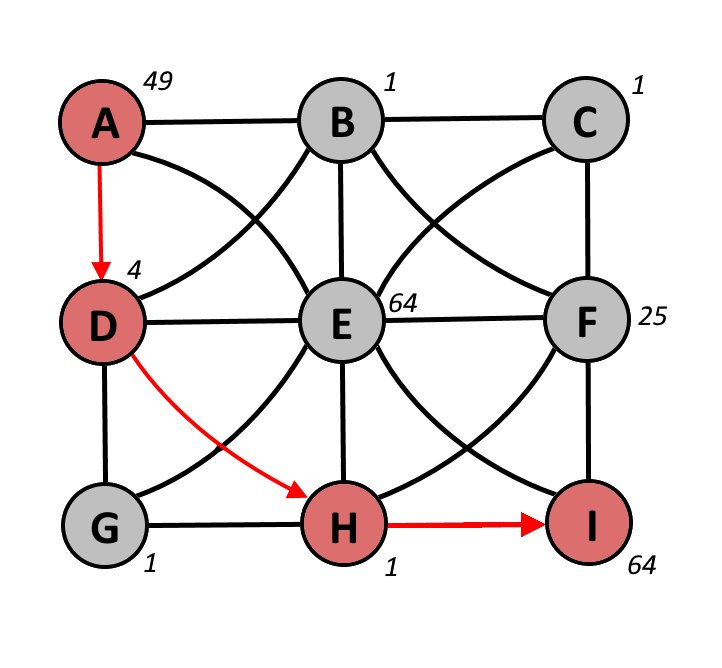
\includegraphics[scale=0.5]{Grafe.png}
\caption{Grafe met het kortste pad aangeduid}
\label{fig:Graph}
\end{figure}

\newpage
\section{Alternatieve Pixeldistance-formule}
We nemen nu een nieuwe afstandsfunctie $ \sqrt{r^2 + g^2} $ i.p.v. de originele functie $ \sqrt{r^2 + g^2 + b^2} $.

De blauwe component wordt nu dus niet meer bekeken bij het berekenen van de afstand tussen twee pixels. Hierdoor zal bijna iedere
afbeelding in de praktijk een snellere uitvoeringstijd kennen, omdat er minder berekeningen gebeuren. Hoe meer blauw er aanwezig is
in een afbeelding, of beter, hoe meer doorslaggevend blauw is voor de grens tussen twee afbeeldingen, hoe simpeler de grens er zal uitzien
als we de nieuwe afstandsfunctie gebruiken. De grens wordt dus versimpeld en de afbeelding zal er anders uitzien.

In een afbeeldingpaar zonder de kleur blauw zal deze nieuwe functie geen effect hebben op de grens. Anderzijds zal het programma geen goede grens vinden tussen
twee afbeeldingen waar enkel de kleur blauw in voorkomt. In dit geval zal het de korste weg in aantal pixels aanduiden als grens.
Dit komt omdat in zo'n afbeeldingenpaar de kost van een pixel altijd gelijk is aan 0, en dus is het gewicht van eenderwelk pad 0. Hierdoor gaat
het algoritme van Dijkstra zoeken naar een kortste pad in aantal pixels, omdat het stopt zodra het de eind-node heeft gevonden.

Het kan echter ook zijn dat dit pad zeer lang is. Dit hangt af van de implementatie van het algoritme. Omdat het gewicht van ieder pad gelijk
is aan 0, zal de PriorityQueue alle paden als \textquotedbl even lang\textquotedbl  zien, alhoewel dat niet altijd zo is. Zo kan het dus ook zijn dat een bepaald
(puur blauw) afbeeldingenpaar een zeer lange uitvoeringstijd heeft omdat de grens voortdurend heen en weer gaat.

\section{Tijdscomplexiteit}

\newpage
\section{Seam en complexe vormen}
Om te voorkomen dat de seam complexere vormen aanneemt kunnen we een simpele aanpassing maken. Voor de volgende node te vinden in het algoritme
van Dijkstra gaan we kijken naar de buren van een bepaalde node. Hier kunnen we onze aanpassing maken door enkel de buren die zich rechts en/of onder
die node bevinden te bekijken. We maken dus een gerichte graaf waarbij alle bogen naar rechts en/of naar onder gericht zijn.

\section{Langste niet-cyclische pad}
Als we het langste niet-cyclishe pad nemen als de grens tussen de twee afbeeldingen in plaats van het kortste pad, dan zal de grens de hele
afbeelding innemen. Het visuele resultaat hangt nu dus af van het algoritme dat de afbeeldingen samenbrengt m.b.v. het masker. Dat masker bestaat
uit enkel de grens en in onze implementatie wordt de grens vervangen met de tweede afbeelding. Het resultaat zal dus de originele tweede afbeelding zijn als
de twee afbeeldingen even groot zijn en er geen offsets gebruikt zijn.

\newpage
\section{Extra voorbeelden}
Onderstaande afbeeldingen zijn nog enkele extra, grappige afbeeldingen van de resultaten van het programma.

In dit eerste resultaat is het duidelijk dat een verschillend gekleurde lijn duidelijk nodig is.
\begin{figure}[h!]
\centering

\includegraphics[scale=0.2]{../myexamples/meme1.png}

\includegraphics[scale=0.2]{../myexamples/meme2.png}
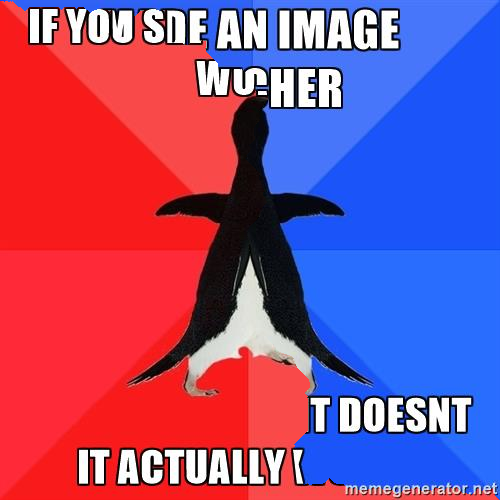
\includegraphics[scale=0.2]{../myexamples/meme-output.png}
\caption{meme1.png, meme2.png en meme-output.png}
\label{fig:Meme}
\end{figure}

Die lijn heb is hier in het groen toegevoegd.
\begin{figure}[h!]
\centering
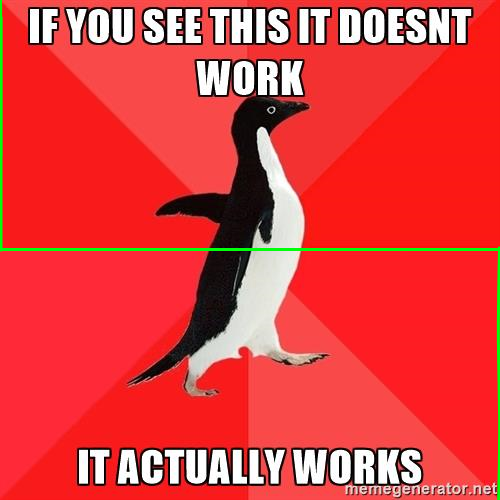
\includegraphics[scale=0.2]{../myexamples/meme1a.png}

\includegraphics[scale=0.2]{../myexamples/meme2a.png}

\includegraphics[scale=0.2]{../myexamples/meme-a-output.png}
\caption{meme1a.png, meme2a.png en meme-a-output.png}
\label{fig:MemeA}
\end{figure}

\end{document}
